\documentclass{beamer}
% \usepackage[utf8]{inputenc}
\usepackage[T1]{fontenc}
\usetheme{CambridgeUS}
\useoutertheme{miniframes}
\usecolortheme{dove}
\usefonttheme{serif}
\beamertemplatenavigationsymbolsempty
\usepackage{lmodern}
\usepackage[scale=2]{ccicons}
\usepackage{tikz}

\setbeamertemplate{background}{\tikz[overlay,remember picture]\node[opacity=0.07]at (current page.center){
\includegraphics[width=8cm]{images/logo-PW.png}};}

\defbeamertemplate{headline}{pwtemplate}{
    \leavevmode%
    \hbox{%
        \begin{beamercolorbox}[wd=\paperwidth,ht=2.25ex,dp=1ex,right]{title in head/foot}%
            \usebeamerfont{title in head/foot}\insertframenumber/\inserttotalframenumber\hspace*{2em}
        \end{beamercolorbox}}%
    \vskip0pt% 
}

\defbeamertemplate{footline}{pwtemplate}{%
    \leavevmode
    \setbeamercolor{lfooterbox}{bg=gray!10}
    \begin{beamercolorbox}[wd=.33\paperwidth,ht=7pt,dp=4pt,center]{lfooterbox}%
        \usebeamerfont{author in head/foot}\insertshortauthor
    \end{beamercolorbox}%
    \setbeamercolor{cfooterbox}{bg=gray!20}
    \begin{beamercolorbox}[wd=.34\paperwidth,ht=7pt,dp=4pt,center]{cfooterbox}%
        \usebeamerfont{date in head/foot}\insertshorttitle
    \end{beamercolorbox}%
    \setbeamercolor{rfooterbox}{bg=gray!10}
    \begin{beamercolorbox}[wd=.33\paperwidth,ht=7pt,dp=4pt,center]{rfooterbox}%
        \usebeamerfont{title in head/foot}\insertshortinstitute
    \end{beamercolorbox}
}


\usepackage[english]{babel}
% \usepackage[english, polish]{babel}

\usepackage{listings}
\lstset{basicstyle=\ttfamily\footnotesize,breaklines=true}
\usepackage{siunitx}
\usepackage{pifont}
\usepackage{amsmath,amssymb,amsfonts}
\usepackage{graphicx}
\usepackage[export]{adjustbox}
\usepackage{float}
\usepackage{xcolor}
\usepackage{setspace}

\newcommand{\todo}[1]{\textcolor{red}{TODO: #1}}

\newcommand{\imagesource}[1]{
    \begin{spacing}{0.5}
        \texttt{\textit{ \tiny{source: #1}}}
    \end{spacing}
}

\newenvironment{columnframe}[1]{
    \begin{frame}[environment=columnframe,fragile]{#1}
        \begin{columns}
            }{
        \end{columns}
    \end{frame}
}




\title[STS]{Silicon Tracking System}
    \subtitle{\textit{at the CBM experiment}}
\author[T. Fic]{Tobiasz Fic}
\institute[WUT]{Warsaw University of Technology}
\date{4 June 2024}

\begin{document}

\setbeamertemplate{headline}{}
\setbeamertemplate{footline}{}

\setbeamertemplate{background}{\tikz[overlay,remember picture]\node[opacity=0.07]at (current page.center){
\includegraphics[width=8cm]{images/logo-PW.png}};}
\begin{frame}
    \maketitle
\end{frame}
\setbeamertemplate{background}{}

\setbeamertemplate{headline}[pwtemplate]
\setbeamertemplate{footline}[pwtemplate]

\begin{columnframe}{GSI and FAIR}
    \begin{column}{0.5\textwidth}
        \begin{figure}
            \centering
            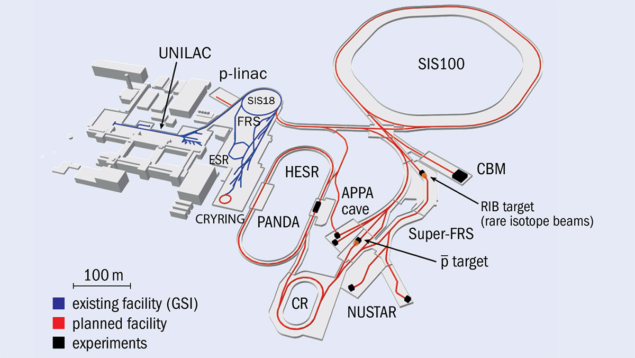
\includegraphics[width=\textwidth, frame]{images/fair_sis100_diagram.jpg}
        \end{figure}
    \end{column}
    \begin{column}{0.5\textwidth}
        \begin{itemize}
            \item one
            \item two
            \item three
        \end{itemize}
    \end{column}
\end{columnframe}

\begin{columnframe}{The CBM Experiment}
    \begin{column}{0.5\textwidth}
        \begin{figure}
            \centering
            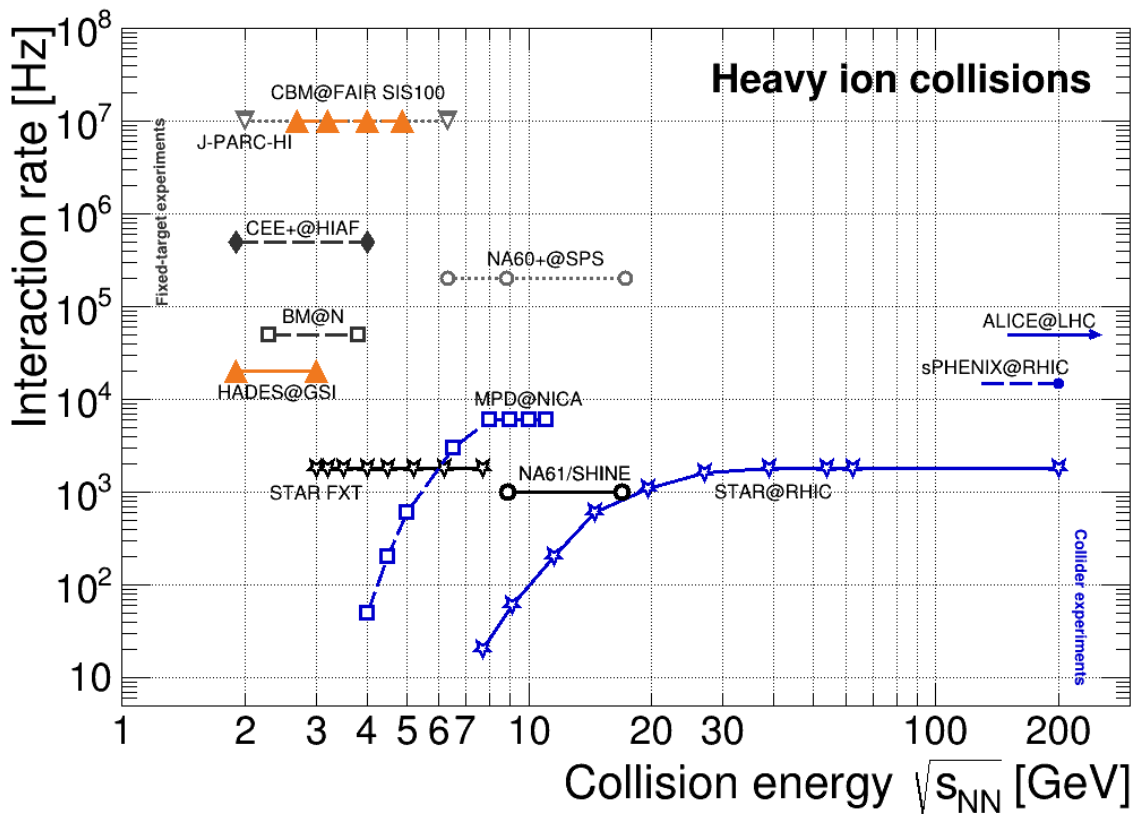
\includegraphics[width=\textwidth, frame]{images/galatyuk_map_of_experiments.png}
        \end{figure}
    \end{column}
    \begin{column}{0.5\textwidth}
        \begin{itemize}
            \item one
            \item two
            \item three
        \end{itemize}
    \end{column}
\end{columnframe}

\begin{columnframe}{The CBM experiment detector setup}
    \begin{column}{0.5\textwidth}
        \begin{figure}
            \centering
            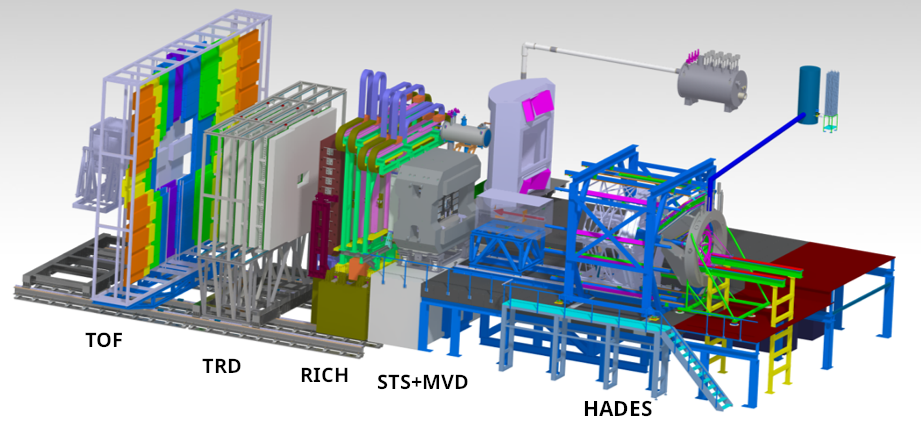
\includegraphics[width=\textwidth, frame]{images/CBM_HADES_new_setup.png}
        \end{figure}
    \end{column}
    \begin{column}{0.5\textwidth}
        \begin{itemize}
            \item one
            \item two
            \item three
        \end{itemize}
    \end{column}
\end{columnframe}

\begin{columnframe}{Silicon Tracking System - goals}
    \begin{column}{0.5\textwidth}
        \begin{figure}
            \centering
            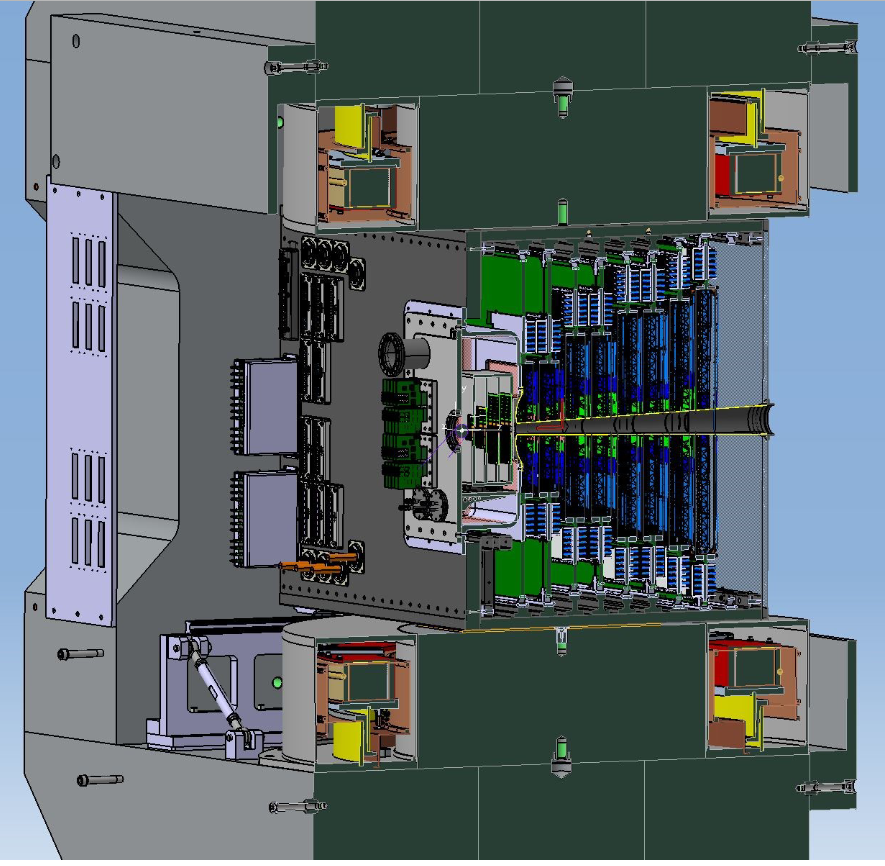
\includegraphics[width=0.6\textwidth, frame]{images/sts_render.png}
        \end{figure}
    \end{column}
    \begin{column}{0.5\textwidth}
        \begin{itemize}
            \item one
            \item two
            \item three
        \end{itemize}
    \end{column}
\end{columnframe}

\begin{columnframe}{Silicon Tracking System - overview}
    \begin{column}{0.5\textwidth}
        \begin{figure}
            \centering
            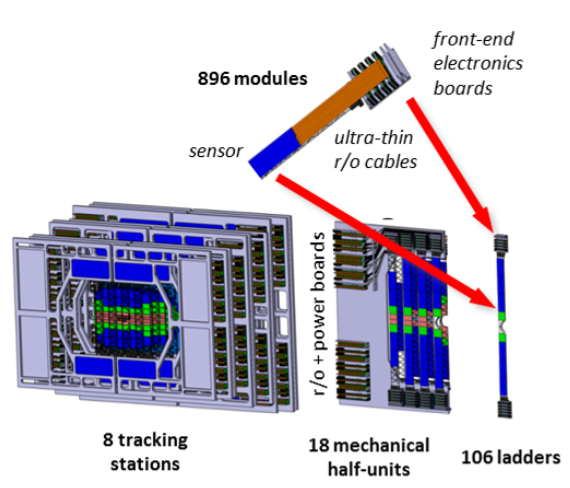
\includegraphics[width=0.9\textwidth, frame]{images/sts_integration_model.png}
        \end{figure}
    \end{column}
    \begin{column}{0.5\textwidth}
        \begin{itemize}
            \item one
            \item two
            \item three
        \end{itemize}
    \end{column}
\end{columnframe}
\begin{columnframe}{STS - Dimensions}
    \begin{column}{0.5\textwidth}
        \begin{figure}
            \centering
            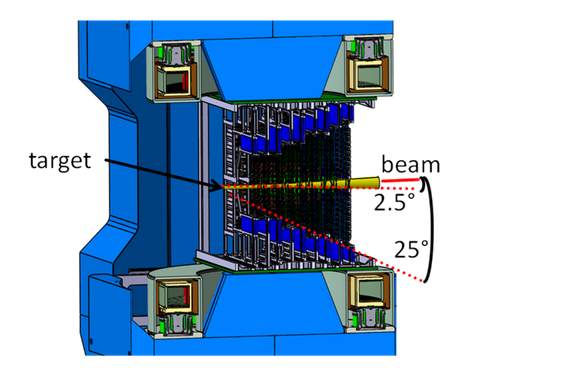
\includegraphics[width=0.6\textwidth, frame]{images/sts_dimensions.png}
        \end{figure}
    \end{column}
    \begin{column}{0.5\textwidth}
        \begin{itemize}
            \item one
            \item two
            \item three
        \end{itemize}
    \end{column}
\end{columnframe}
\begin{columnframe}{STS - silicon sensors}
    \begin{column}{0.5\textwidth}
        \begin{figure}
            \centering
            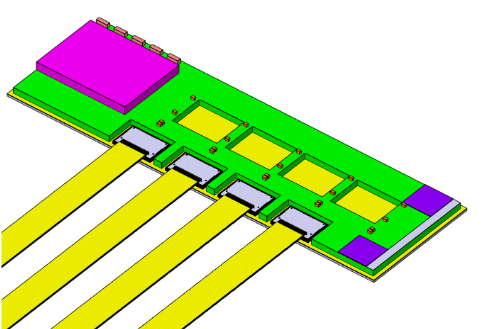
\includegraphics[width=0.6\textwidth, frame]{images/sts_strips_1.png}
            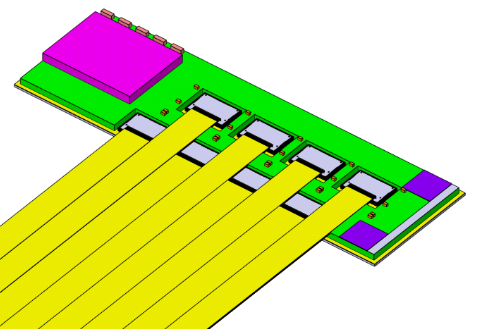
\includegraphics[width=0.6\textwidth, frame]{images/sts_strips_2.png}
        \end{figure}
    \end{column}
    \begin{column}{0.5\textwidth}
        \begin{itemize}
            \item one
            \item two
            \item three
        \end{itemize}
    \end{column}
\end{columnframe}
\begin{columnframe}{STS - calibration}
    \begin{column}{0.5\textwidth}
        \begin{figure}
            \centering
            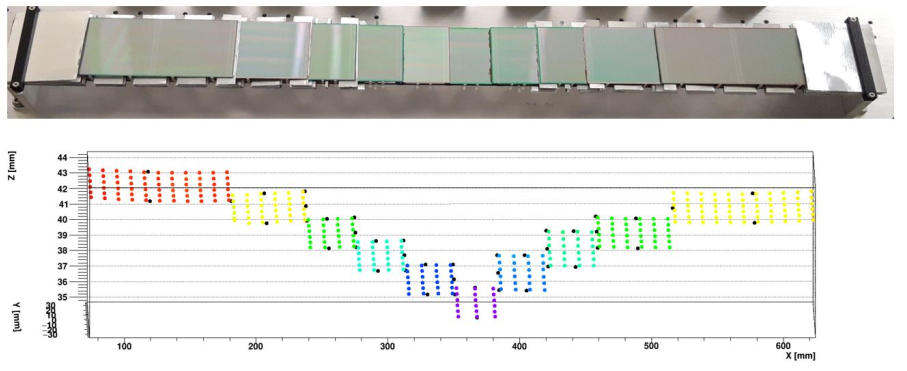
\includegraphics[width=\textwidth, frame]{images/sts_strips.png}
        \end{figure}
    \end{column}
    \begin{column}{0.5\textwidth}
        \begin{itemize}
            \item one
            \item two
            \item three
        \end{itemize}
    \end{column}
\end{columnframe}

\begin{columnframe}{STS - reconstruction}
    \begin{column}{0.5\textwidth}
        \begin{figure}
            \centering
            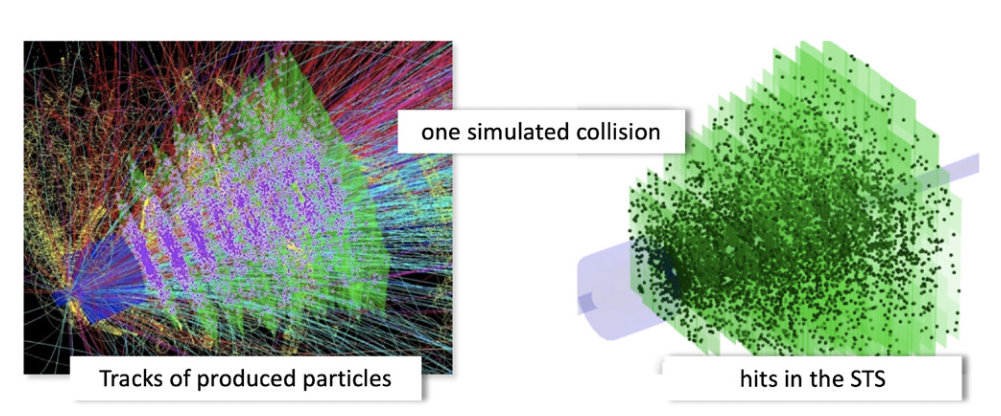
\includegraphics[width=0.6\textwidth, frame]{images/sts_reco.png}
        \end{figure}
    \end{column}
    \begin{column}{0.5\textwidth}
        \begin{itemize}
            \item one
            \item two
            \item three
        \end{itemize}
    \end{column}
\end{columnframe}

\begin{columnframe}{STS - expansion (MVD)}
    \begin{column}{0.5\textwidth}
        \begin{figure}
            \centering
            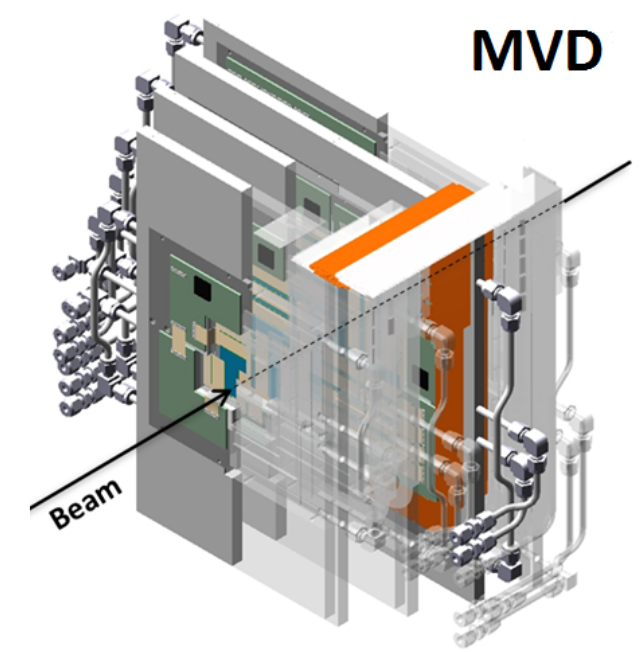
\includegraphics[width=0.6\textwidth, frame]{images/mvd_render.png}
        \end{figure}
    \end{column}
    \begin{column}{0.5\textwidth}
        \begin{itemize}
            \item one
            \item two
            \item three
        \end{itemize}
    \end{column}
\end{columnframe}

\begin{columnframe}{STS - current state (mCBM)}
    \begin{column}{0.5\textwidth}
        \begin{figure}
            \centering
            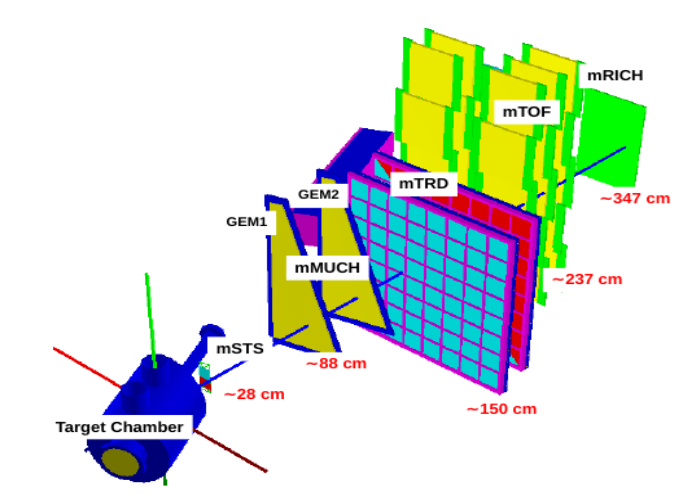
\includegraphics[width=0.6\textwidth, frame]{images/mCBM_render.png}
        \end{figure}
    \end{column}
    \begin{column}{0.5\textwidth}
        \begin{itemize}
            \item one
            \item two
            \item three
        \end{itemize}
    \end{column}
\end{columnframe}


\begin{columnframe}{Outlook}
    \begin{column}{0.5\textwidth}
        \begin{figure}
            \centering
            
\includegraphics[width=0.6\textwidth, frame]{images/pusheen.png}
        \end{figure}
    \end{column}
    \begin{column}{0.5\textwidth}
        \begin{itemize}
            \item one
            \item two
            \item three
        \end{itemize}
    \end{column}
\end{columnframe}


\setbeamertemplate{headline}{}
\setbeamertemplate{footline}{}
\begin{frame}{}
    \centering
    \Large{Thank you for your attention}
\end{frame}

\end{document}